\section{Praktikos veiklos aprašymas}

\subsection{Projektas}
Kaip buvo minėta ankščiau, profesinės praktikos metu visi darbai buvo vykdomi su „Bitė Lietuva“ vidinė klientų aptarnavimo informacinė sistema.
„Bitė Lietuva“ yra įmonės nuolatinis klientas, 2018 metais „INVENTI“ sukūrė šią sistemą \cite{medus}, ir integravo su egzistuojančiomis „Bitė Lietuva“ sistemomis.
Sistema įmonės viduje turi kodinį pavadinimą „medus“ \ref{img:medus}.
Klientui „Bitė Lietuva“ atsirado poreikis atlikti televizijos paslaugų pardavimą per šią sistemą, tam kad galutinis vartotojas galėtų naudotis
„Go3 | BITĖ“ televizijos paslaugomis \cite{go3}. „INVENTI“ pasirašė sutartį atlikti šį projektą dviem etapais.
Taip pat prie projekto prisijungė ir kiti vendoriai - įmonė „Baltic Amadeus“. Dėl COVID-19 grėsmės, „Bitė Lietuva“ siūlo televizijos paslaugomis 3 mėnesius naudotis nemokamai.


\begin{figure}[H]
    \centering
    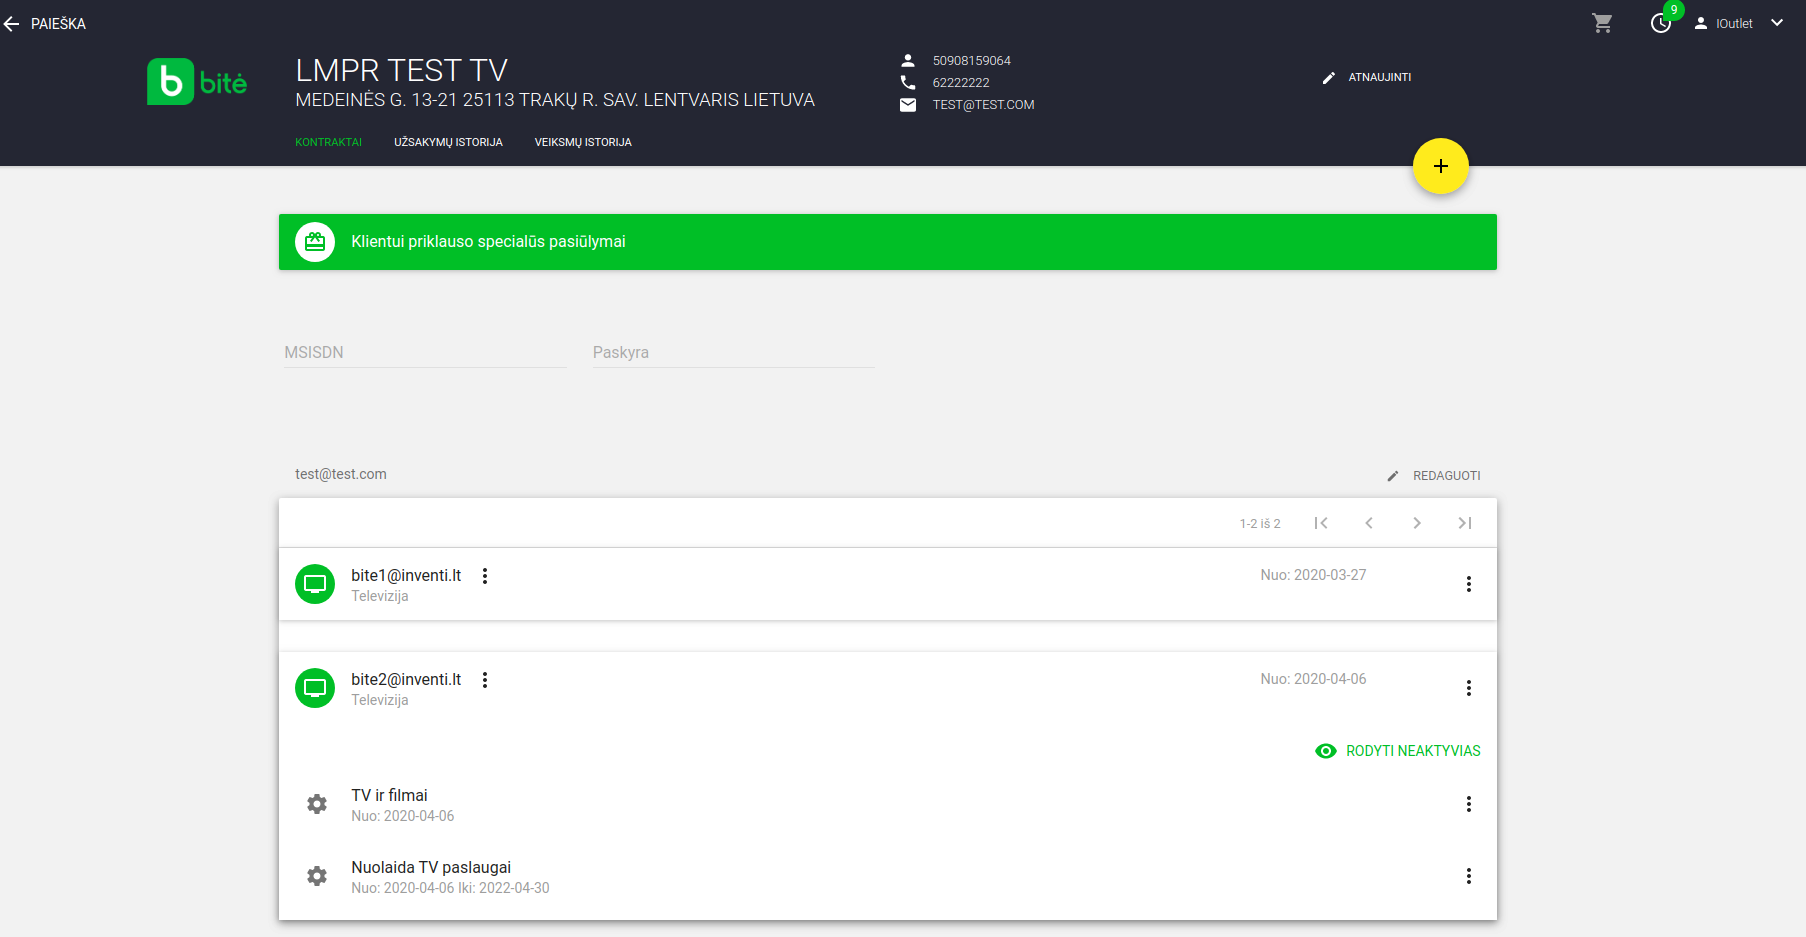
\includegraphics[scale=0.25]{img/medus.png}
    \caption{Vidinės klientų aptarnavimo sistemos vartotojo sąsaja.}
    \label{img:medus}
\end{figure}

\subsection{Darbo procesas}
Prieš pradedant projektą, komanda atlieka kliento pateiktų vartotojų istorijų analizę, išskaido jas į užduotis, kiekvieną užduotį įvertina, ir sudeda į projekto neatliktų užduočių sąrašą.
Darbas vykdavo pagal agile metodologiją, kas dvi savaites planuojami sprintai. Sprinto planavimo metu, visa komanda susirenka ir padaro atliktų užduočių apžvalgą „Jira“
užduočių projekto sistemoje, apžvelgiama, kokios užduotys buvo atliktos praeitame sprinte, o kurios keliauja į naują.
Atlikus peržiūrą, praeitas sprintas uždaromas, atidaromas naujas. Neužbaigtos užduotys perkeliamos į naują sprintą, ir tada atliekama neatliktų užduočių sąrašo analizė.
Iš neatliktų užduočių sąrašo, užduotys perkeliamos į naują sprintą pagal svarbumo prioritetą, tol, kol nebus viršytas dviejų savaičių darbo valandų limitas. Įmonėje taikoma praktika,
kad programuotojas programavimo darbams vidutiniškai skiria 6 valandas, 2 valandos lieka susitikimams, pokalbiams su klientu, arba kitai, su programavimu nesusijusiai veiklai.
Pirmadieniais vykdavo susitikimas, kurio metu buvo uždaromas praeitas sprintas ir buvo planuojamas naujas.

Kiekviena diena ryte vyksta „stand-up“ susitikimai, dažniausiai tai konferencinis pokalbis su klientu ir kitais vendoriais, bet kartais tekdavo vykti pas klientą į ofisą, kur šie
susitikimai vykdavo gyvai. Kiekvienas „stand-up“ dalyvis trumpai nupasakoja, ką praeitą dieną nuveikė, su kokiomis problemomis susidūrė ir kaip jas sprendė.
Šie susitikimai dažniausiai užtrunka 15 minučių, po jų seka komandos vidiniai komandos pasitarimai.

Programavimo darbai prasideda nuo „Jira“ užduoties statuso pakeitimo, kurį pradėjus darbą reikia pakeisti į „in progress“. Programavimo darbams sukuriama nauja GIT šaka, kurios pavadinimas
- užduoties numeris. Atlikus programavimo darbus, kodo versijavimo sistemoje
sukuriamas „merge request“ į vykdomo projekto šaką, kurio paskirtis - kodo peržiūra. Kodo peržiūras atlieka kiti komandos programuotojai, peržiūrėjus kodą, savo pastabas surašo
„Gitlab“ versijavimo sistemoje. Jeigu pastabų nėra - duodamas leidimas atlikti šakų suvienijimą. Tada galima pakeisti užduoties statusą į „done“.
Kai visos užduotys, priklausančios tam tikrai vartotojo istorijai yra užbaigtos,
prašomas kliento leidimas sudiegti PĮ pakeitimus į testinę aplinką, kurioje kliento testuotojai galėtų ištestuoti naują funkcionalumą.

Jeigu funkcionalumas turi klaidų - testuotojai užregistruoja jas „Phabricator“ sistemoje. Iš šios sistemos, jos perkeliamos į „Jira“ sistemą, atliekami klaidų taisymo darbai, pataisymai
sukeliami į testinę aplinką, kol galiausiai įgyvendintas funkcionalumas atitinka specifikuotam reikalavimuose. Kai yra įgyvendintas tam tikras funkcionalumo paketas, planuojamas
išleidimas (angl. „release“) į produkcinę aplinką. Kai visas naujas funkcionalumas pilnai ištestuotas, ir regresinis testavimas neatranda klaidų - naujo funkcionalumo paketas
sudiegiamas į produkcinę aplinką. Šie diegimai atliekami vidutiniškai kartą per mėnesį.


\subsection{Projekte naudojamos technologijos}
Kaip jau buvo minėta ankščiau, sistemos UI dalis yra parašyta su JavaScript kalba, naudojama „React“ biblioteka. Vartotojo sąsajai naudojama „Material UI“ biblioteka.
UI aplikacija su serverine dalimi bendrauja naudojant tarpinį serverį - „Nginx“.
Sistemos serverinė dalis parašyta su Java programavimo kalba, naudojamas „Spring“ programavimo karkasas. Serverinė dalis yra
įgyvendina mikroservisų architektūrinį principą. Servisai tarpusavyje apsikeičia duomenimis per
REST arba SOAP sąsają. Du servisai, daugiausiai bendraujantys su UI, įgyvendina naudojant CQRS architektūrinį principą,
kuris atskiria duomenų įrašymo ir duomenų užklausų sluoksnius. Vienas servisas atsakingas už užsakymų krepšelio valdymą, sistemoje įgyvendinta didelė aibė skirtingų procesų \ref{img:options},
kurie vykdomi per užsakymų krepšelį. Kitas servisas atsakingas krepšelio apdorojimą, iš gautų duomenų sugeneruojami sutarties duomenys, kurie nukeliauja į vidinę apskaitos sistemą.
Žinutėms (angl. „events“) tarp servisų naudojamas žinučių brokeris „Apache Kafka“. Kadangi servisas, bendraujantis su apskaitos sistema naudoja SOAP protokolą, buvo sukūrtas
servisas, kurio paskirtis - gaunamas REST užklausas, naudojant „Apache Camel“ technologiją, paversti į SOAP užklausas, ir perduoti dedikuotam servisui.
Taip pat yra ir kiti servisai, turintys po vieną paskirtį, pavyzdžiui, vienas servisas atsakingas už „PDF“ sutarčių generavimą, kitas - už el. laiškų siuntimą ir t.t.
Kadangi „Bitė Lietuva“ priklauso „Bitė“ grupei, kurioje taip pat vykdo veiklą įmonė „Bitė Latvija“, tam tikri servisai veikia tik vienos šalies aplinkose.

\begin{figure}[H]
    \centering
    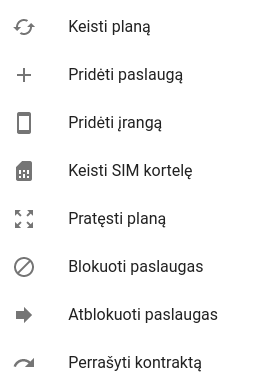
\includegraphics[scale=0.4]{img/options.png}
    \caption{Galimi kliento sutarties procesai.}
    \label{img:options}
\end{figure}

Mikroservisų architektūros valdymui naudojama konteinerių technologija „Docker“, kuri leidžia programų kūrėjams ir sistemų administratoriams lengvai ir greitai
talpinti aplikacijas konteineriuose, kurie izoliuoti nuo operacinės sistemos. Konteinerizuotos aplikacijos diegimui naudojama „Kubernetes“ konteinerių orkestravimo technologija.
Ši technologija leidžia koreguoti resursus pagal poreikį, lengvai atnaujinti PĮ versijas, apdoroti žurnaliavimą ir t.t.
